\documentclass[aspectratio=169]{beamer}
\usepackage{pres_preamble}
\usetheme{UiB}


%----------------------------------------------------------------------------------------
%	TITLE PAGE
%----------------------------------------------------------------------------------------

\title{Differential and Symplectic Geometry}

\author{Clayton Shonkwiler and Patrick Shipman}
\setbeamercolor{title}{fg=white} 
\setbeamercolor{subtitle}{fg=white} 


%----------------------------------------------------------------------------------------
%	PRESENTATION SLIDES
%----------------------------------------------------------------------------------------

\begin{document}
 
    \begin{frame}{}
\vfill
        \begin{figure}
            \centering
            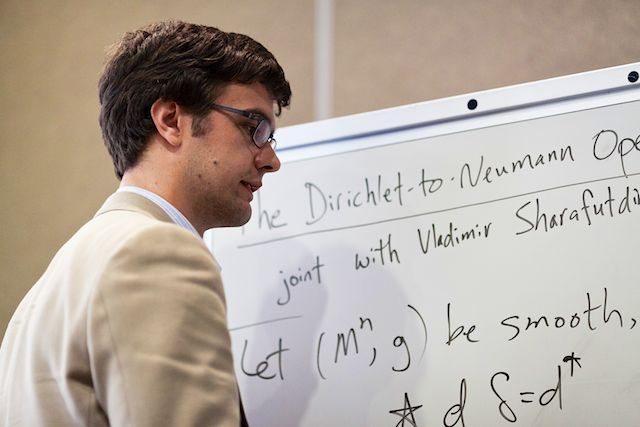
\includegraphics[width=.7\textwidth]{clay.jpg}
			\caption{Clayton Shonkwiler}
        \end{figure}\vfill
    \end{frame}
    
    
    \begin{frame}{Interests}
\vfill
        \begin{itemize}
            \item Differential and symplectic geometry.
            \item Applications to synthetic chemistry, polymer physics.
            \item Polygon spaces and geometric probability/measure.
			\item Relationship of symplectic geometry to frame theory.
			\item Differential forms and the geometric inverse problems.
        \end{itemize}
\vfill
    \end{frame}

    \begin{frame}{}
\vfill
\begin{figure}[H]
     \centering
     \begin{subfigure}[b]{0.45\textwidth}
         \centering
    	
\includegraphics[width=\textwidth]{33700724514_35273ae7ca_b.jpg}
     \end{subfigure}
     \hfill
     \begin{subfigure}[b]{0.45\textwidth}
         \centering
         
\includegraphics[width=\textwidth]{download.png}
     \end{subfigure}
\caption{Check out \url{shonkwiler.org}, @shonk on Instragram, and \url{community.wolfram.com/web/claytonshonkwiler}}
\end{figure}
\vfill
    \end{frame}

       \begin{frame}{}
\vfill
        \begin{figure}
            \centering
            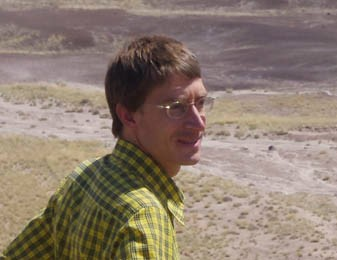
\includegraphics[width=.6\textwidth]{patrick.jpg}
			\caption{Patrick Shipman}
        \end{figure}
\vfill
    \end{frame}

    \begin{frame}{(Relevant) Interests}
\vfill
        \begin{itemize}
            \item Differential geometry.
            \item Applications to organic systems and pattern formation.
            \item Dirac operator and minimal surfaces.
			\item Geometric approaches to ODEs and PDEs.
        \end{itemize}
\vfill
    \end{frame}
   
    \begin{frame}{}
\vfill
\begin{figure}[H]
     \centering
     \begin{subfigure}[b]{.7\textwidth}
         \centering
    	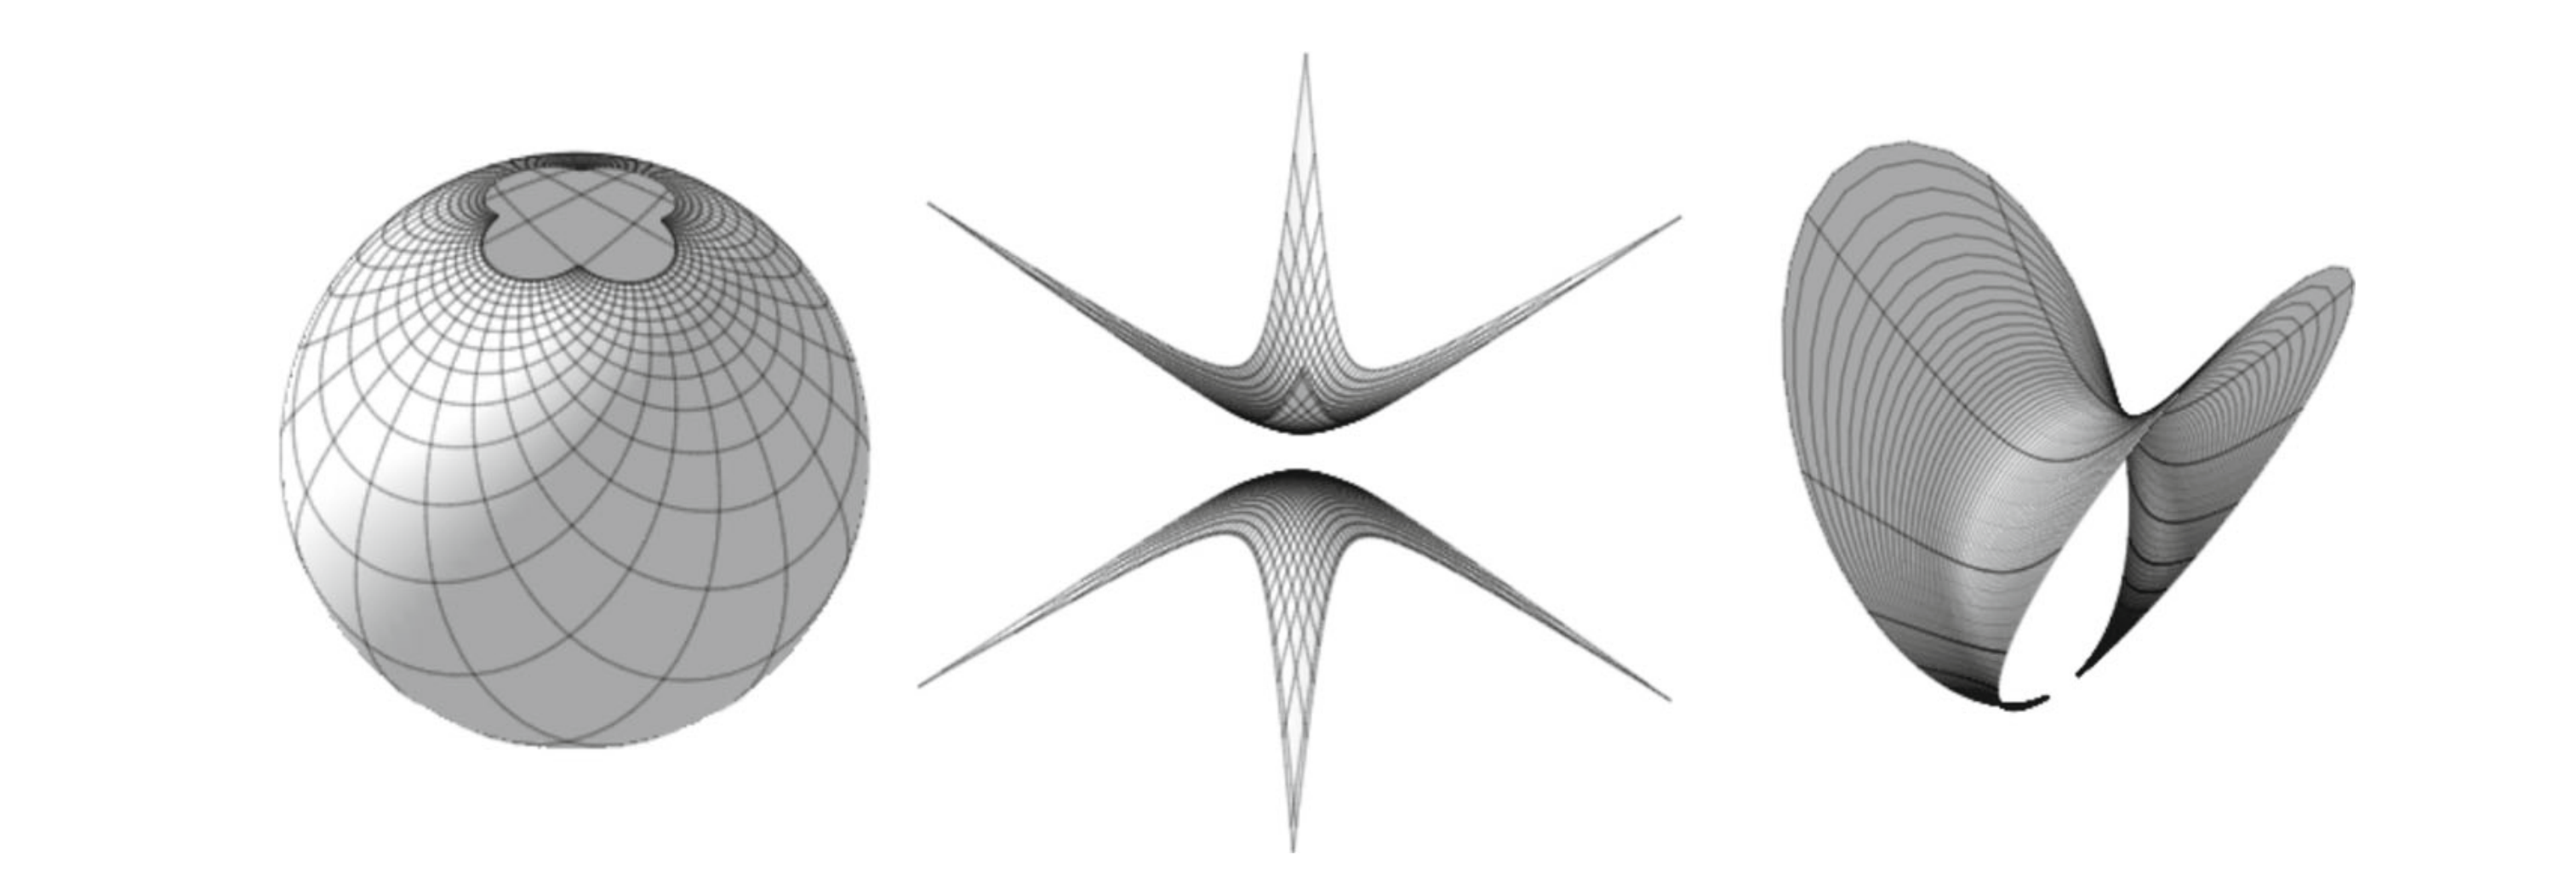
\includegraphics[width=\textwidth]{weierstrass_enneper.png}
     \end{subfigure}
     \\
     \begin{subfigure}[b]{.7\textwidth}
         \centering
         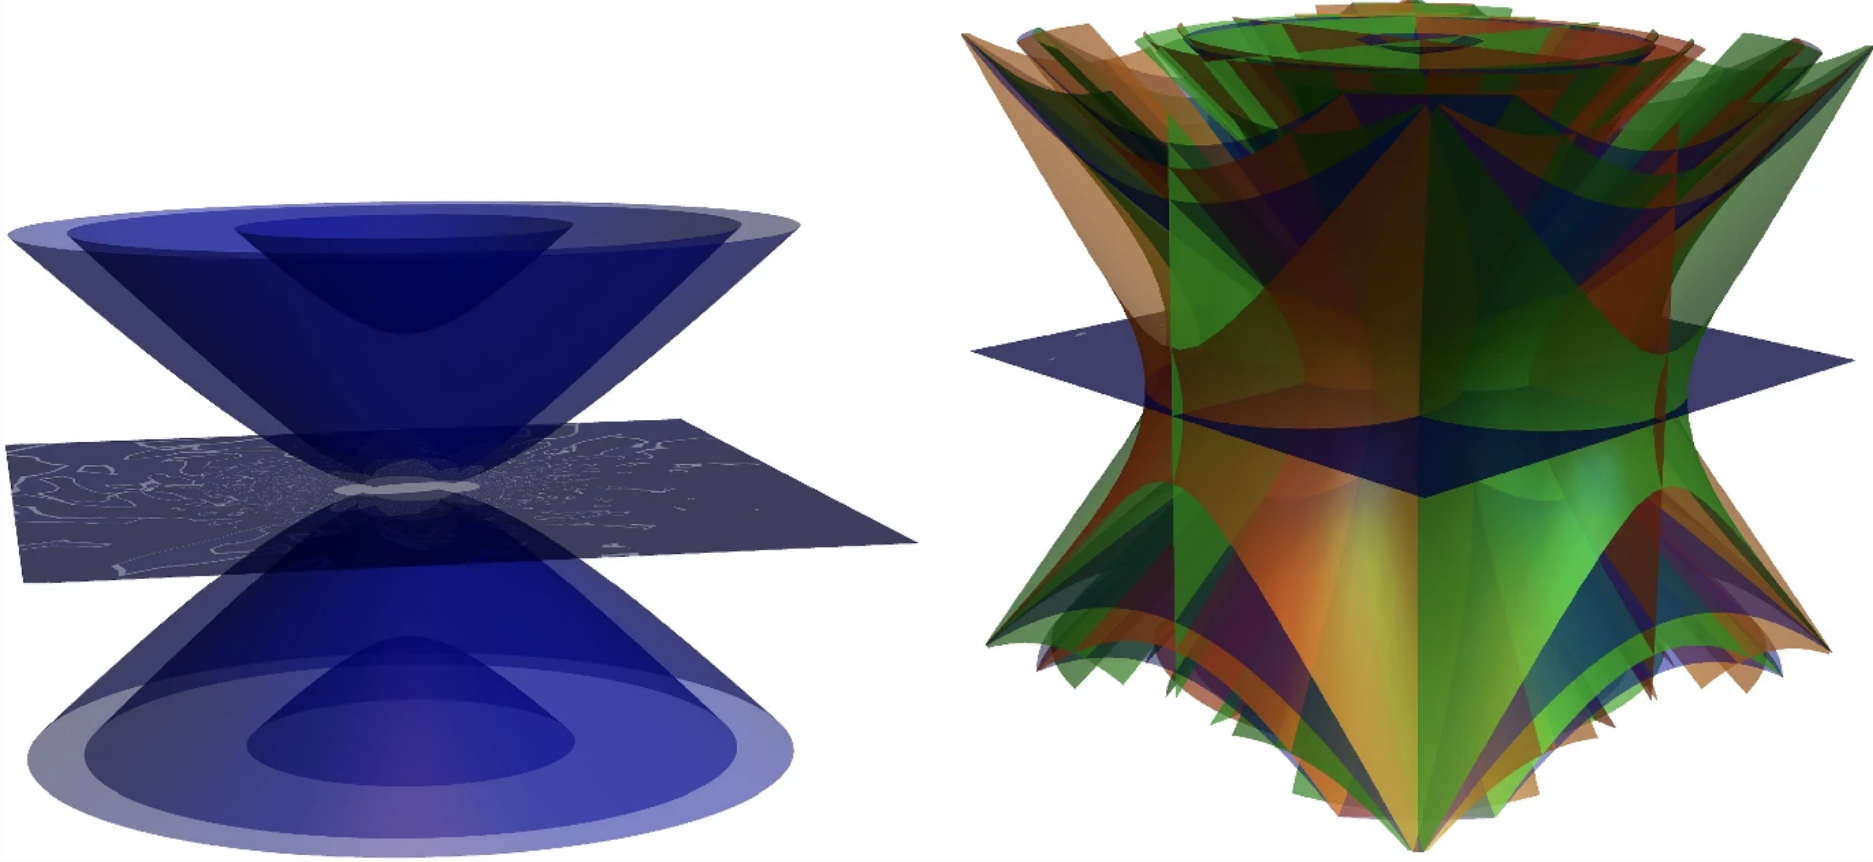
\includegraphics[width=\textwidth]{conformal.png}
     \end{subfigure}
\end{figure}
\vfill
    \end{frame}

\end{document}

%
%

%\section{Plasma Fluids}
%

%
%\begin{frame}{Classical Fluid Quantities}
%\vfill
%    \begin{itemize}
%        \item Vorticity $\blade{\omega}$ represents rotational fluid motion in a plane
%        \begin{figure}
%    \centering
%    \begin{subfigure}[b]{0.15\textwidth}
%        \centering
%        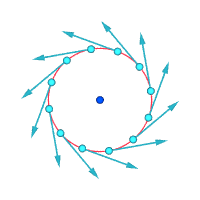
\includegraphics[width=\textwidth]{figures/Vorticity_Figure_01_c.png}
%    \end{subfigure}
%    \hspace*{3cm}
%    \begin{subfigure}[b]{0.15\textwidth}
%        \centering
%        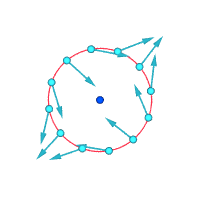
\includegraphics[width=\textwidth]{figures/Vorticity_Figure_02_c.png}
%    \end{subfigure}
%    \end{figure}
%        \item In general, the product of velocity with vorticity decomposes
%        \[
%        \blade{v}\blade{\omega} = \underbrace{\blade{v}\cdot \blade{\omega}}_{\textrm{transport}}+\underbrace{\blade{v}\wedge\blade{\omega}}_{\textrm{helicity}}
%        \]
%            
%        \begin{figure}
%            \centering
%            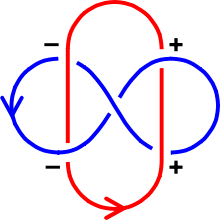
\includegraphics[width=0.15\textwidth]{figures/gauss_linking.png}
%        \end{figure}
%    \end{itemize}
%
%\vfill    
%\end{frame}
%
%%%%%%%%%%%%%%%%%%%%%%%%%%%%%%%%%%%%%%%%%%%%%%%%%%
%

%

%
%\begin{frame}{Plasma Fluid}
%    
%\end{frame}
%